% Blind symbolic interpretation of CMB beta-VAE latent spaces.
% ARCHIVED DRAFT (superseded): see README.md in this directory. Drafted from
% docs/results_compendium.md (commit cb1221a); every number is T2-confirmed
% and traces to a consolidated deliverable in experiments/. Predates the
% stage-2 audit; states a decoder-side -2 readout that was later withdrawn.
% Compile: pdflatex main && pdflatex main   (figures via \graphicspath below)
\documentclass[twocolumn,10pt]{article}

\usepackage[margin=1.8cm,columnsep=0.7cm]{geometry}
\usepackage{amsmath,amssymb}
\usepackage{graphicx}
\graphicspath{{../../../figures/}{../../../experiments/}}
\usepackage{booktabs}
\usepackage{microtype}
\usepackage[numbers,sort&compress]{natbib}
\setlength{\bibsep}{2pt}
\usepackage{caption}
\captionsetup{font=small,labelfont=bf,skip=4pt}
\usepackage{xcolor}
\usepackage[colorlinks=true,linkcolor=blue!50!black,citecolor=blue!50!black,urlcolor=blue!50!black]{hyperref}

% --- notation ---------------------------------------------------------------
\newcommand{\As}{A_\mathrm{s}}
\newcommand{\ns}{n_\mathrm{s}}
\newcommand{\omB}{\omega_\mathrm{b}}
\newcommand{\omC}{\omega_\mathrm{cdm}}
\newcommand{\Hz}{H_0}
\newcommand{\lnAs}{\ln A_\mathrm{s}}
\newcommand{\etaS}{\eta_S}
\newcommand{\etapost}{\hat\eta_\mathrm{post}}
\newcommand{\Einv}{E_\mathrm{inv}}
\newcommand{\RSR}{R_\mathrm{SR}}
\newcommand{\MI}{\mathrm{MI}}
\newcommand{\combo}{\As e^{-2\tau}}

% pack floats tighter (avoids a lone trailing float page)
\renewcommand{\topfraction}{0.92}
\renewcommand{\dbltopfraction}{0.92}
\renewcommand{\textfraction}{0.06}
\renewcommand{\floatpagefraction}{0.8}
\setcounter{topnumber}{3}
\setcounter{dbltopnumber}{3}

\title{\bfseries Blind symbolic interpretation of CMB $\beta$-VAE latent spaces:\\
mutual-information regression rediscovers $\combo$}

% TODO: replace with the real author block before submission
\author{Author name(s) here\\
\small Institute, University of Cambridge\\
\small \texttt{zx332@cam.ac.uk}}
\date{Draft of 2026-08-14 --- compiled from \texttt{docs/results\_compendium.md}}

\begin{document}
\maketitle

\begin{abstract}
\noindent
$\beta$-VAE compressions of CMB power spectra learn latents that correlate
with physical parameters, but turning a latent into an \emph{equation} usually
leaks the answer into the analysis (hand-coded reference combinations,
calibration-aware losses, post-hoc latent selection). We present a
pre-registered, fully blind alternative: symbolic regression whose inner loss
and selection metric are both mutual-information estimators --- invariant
under any bijection of either variable --- applied to every latent of two CMB
$\beta$-VAE checkpoints (TT-only; TT+low-$\ell$EE). No derived parameter
combination is computed anywhere in the pipeline; all thresholds were frozen
before unblinding, with the amplitude sector as internal positive control.
The search blindly recovers the textbook combination $\ln(\combo)$; the $-2$
exponent is read out four independent ways (discovered forms; derivative
ratio $-1.974\pm0.018$ / $-1.993\pm0.008$; an answer-agnostic ratio detector,
$-2.000$; decoder templates, $-1.87$) and reappears, unsolicited, in another
latent's residual. All 11 latents receive validated symbolic ``cards'' --- a
primary coordinate saturating its blindly selected support ($\etaS\approx1$)
plus a discovered second coordinate --- with 10/11 ``primarily interpreted''
and one honest failure. Symbolic structure does not terminate at two levels:
every stage-2 residual remains structured, robustly to an interaction-aware
ansatz. The protocol --- freeze, validate on a positive control, unblind,
a null for every instrument --- is a reusable recipe for interpreting
scientific latent spaces.
\end{abstract}

\section{Introduction}
\label{sec:intro}

Neural compressions of cosmological observables now routinely learn latent
spaces whose coordinates \emph{look} physical: a $\beta$-VAE trained on CMB
temperature power spectra organises its most informative latent along the
amplitude direction, and correlation with hand-picked parameter combinations is
the standard way this is shown \citep{piras2025}. That last step is where
interpretability claims become circular. If the analyst computes
$\combo$ and correlates it with a latent, the pipeline contains the answer; if
a symbolic fit is scored by mean-squared error against the standardised latent,
the search is rewarded for reproducing the encoder's calibration, not for
finding its content.

This paper asks --- and answers --- a narrower, sharper question: \emph{can the
symbolic content of every latent be recovered with no hint of the answer
anywhere in the pipeline, under pre-registered decision rules?} Our
contributions are methodological first and cosmological second:

\begin{enumerate}\itemsep2pt
\item \textbf{A blind search objective.} Symbolic regression
  (PySR~\cite{cranmer2023}) over \emph{raw} $\Lambda$CDM parameters only, scored
  inside the search loop by a fast Gaussian-mixture mutual-information (MI)
  estimator and post hoc by an independent held-out MI estimate
  \citep{piras2023}. Both are invariant under bijections of either variable, so
  the search can only be rewarded for functional dependence
  (\S\ref{sec:objective}).
\item \textbf{A pre-registered protocol with falsifiable gates.} Every
  threshold was frozen before unblinding the non-amplitude latents; the
  machinery had to first \emph{rediscover} known physics on the amplitude
  sector --- and honestly report what it does not explain --- before any
  discovery claim was allowed (\S\ref{sec:prereg}). Blind-analysis practice of
  this kind is standard in particle physics \citep{klein2005} but rare in
  representation interpretation.
\item \textbf{Results.} The reionization $-2$ recovered blindly four ways
  (\S\ref{sec:minus2}); a validated symbolic card for each of the 11 latents in
  two checkpoints (\S\ref{sec:cards}); model-level structure --- degeneracy
  breaking visible before any regression, a split (not duplicated) amplitude
  sector, and a symbolic hierarchy that does not terminate
  (\S\ref{sec:structure}--\ref{sec:hierarchy}).
\end{enumerate}

We deliberately do not revisit what is established elsewhere --- VAE
architecture, training, and emulation accuracy are those of the reproduction
of Piras et al.~\cite{piras2025}, and symbolic regression
\citep{schmidt2009,cranmer2020} is used off the shelf; the novelty is the
interpretation protocol and what it finds.

\section{Method}
\label{sec:method}

\subsection{Targets, data, and what ``blind'' means}
\label{sec:setup}

Two stored $\beta$-VAE checkpoints are interpreted \emph{as found}, without
retraining: a TT-only convolutional VAE with $L{=}5$ latents, and a
TT+low-$\ell$EE dual-encoder VAE with $L{=}6$ (both $\beta=3\times10^{-4}$,
training seed 42), from an independent PyTorch reproduction of
Piras et al.~\cite{piras2025}. Training data are 500k Latin-hypercube samples of
$\theta=(\omB,\omC,\Hz,\tau,\ln 10^{10}\As,\ns)$ mapped to CLASS spectra
\citep{class2011}. The regression target for latent $k$ is the encoder
posterior mean $\mu_k(\theta)$ over the 50k-row test split; the cached
posterior variances give the stochastic latent $Z_k$ and hence each latent's
finite information ceiling $\MI(Z_k;\theta)$ (\S\ref{sec:ladder}). The test
split is tiered once and for all: T0 (5k rows) for the searches, T1 (20k) for
calibration and audits, T2 (25k) touched only for confirmatory numbers.

Blindness is enforced structurally, not by good intentions:
(i)~\emph{inputs are the six raw parameters only} --- no derived combination
($\combo$ or otherwise) is computed anywhere in the pipeline;
(ii)~\emph{both the inner loss and the selection metric are MI estimators},
so no stage rewards matching the latent's scale or calibration;
(iii)~\emph{latent roles are assigned before any regression} by a
disentanglement audit that measures MI between each latent and each raw
parameter --- the amplitude latents (TT $z_2$, EE $z_5$) are identified from
raw-parameter loadings alone.

\subsection{Mutual information as the search objective}
\label{sec:objective}

PySR searches expressions $f(\theta_S)$ over a support $S$, with unary
operators $\{\exp,\log,\mathrm{neg},\mathrm{square}\}$ and binary
$\{+,-,\times,\div\}$, 200 iterations, 15 populations, maximum complexity 20,
on 5\,000 rows (4\,000 fit / 1\,000 validation), five independent seeds per
configuration. The inner loss is $\exp[-\widehat\MI(f(\theta),\mu_k)]$ with
$\widehat\MI$ a two-component Gaussian-mixture estimator written in pure Julia
(EM on 300-sample sub-batches, milliseconds per call, $\sim$80$\times$ faster
than calling a Python estimator across the language boundary; $\sim$5 min per
seed at 16 threads). Selection is post hoc: every Pareto-front equation is
re-scored with the full \texttt{gmm-mi} estimator \citep{piras2023} on held-out
rows.

The key property is shared invariance. For any bijections $a,b$,
$\MI\!\left(a(f),\,b(\mu_k)\right)=\MI(f,\mu_k)$, so the affine form
$\As(\tau-c)$, the literal $\combo$, and $2\tau-\lnAs$ carry identical scores,
and PySR's parsimony penalty arbitrates among them. The search is therefore
rewarded purely for finding \emph{which function of $\theta$ the latent is},
never for reproducing how the encoder happens to scale it. A practical
corollary found in a 12-configuration hyperparameter sweep: the top-of-front MI
is a capacity dial (it grows with any search-size knob), while the
budget-matched readout MI at complexity $\le$10 is flat across every knob ---
so we \emph{search big and slice small}, reading results at a one-standard-error
knee of the cumulative Pareto envelope rather than at the front's argmax
(Fig.~\ref{fig:envelopes}).

\subsection{Pre-registration, gates, and controls}
\label{sec:prereg}

All decision rules --- sufficiency levels, knee definition, semantic-cluster
equivalence, recurrence thresholds, subset minimality, residual-audit and
level-set pass criteria, and the final status predicates --- were frozen in the
roadmap document \emph{before} unblinding any non-amplitude latent. The
amplitude sector then served as gate G1, a registered positive control: the
frozen instruments had to rediscover the $\{\As,\tau\}$ support, the $-2$
exponent, and support saturation $\etaS\approx1$, \emph{and} correctly report
that the primary coordinate leaves a structured residual (an honesty check
--- instruments that fabricate sufficiency would fail it). G1 passed on both
models. Post-freeze judgement calls were not made silently: five deviations
(e.g.\ the seed tolerance used by recurrence scoring, the additive-hierarchy
limit at the TT amplitude latent) are recorded in a register and printed on the
affected cards. Every instrument ships a null (Table~\ref{tab:controls}):
shuffled targets for the searches, permutation nulls for the residual audits,
shuffled residuals for stage two, shuffled-form and wrong-latent controls for
the level sets, shuffled probes for the subspace analysis.

\begin{table*}[t]
\centering\small
\caption{The instrument ladder. Each row is one frozen instrument; later rows
consume earlier rows' outputs. MI estimates use \texttt{gmm-mi} on held-out
tiers; every decision statistic is compared against the listed null.}
\label{tab:ladder}
\begin{tabular}{@{}p{3.4cm}p{4.7cm}p{4.6cm}p{3.4cm}@{}}
\toprule
Instrument & Question it answers & Decision statistic & Null / control \\
\midrule
Disentanglement audit & which raw parameters does $z_k$ carry? & $\MI(z_k;\theta_j)$ matrix & --- \\
Blind SR (\S\ref{sec:objective}) & which function of $\theta$ is $\mu_k$? & held-out MI of Pareto forms & shuffled target \\
Plateau/knee readout & where does the front saturate? & envelope plateau, 1-SE knee $c^*$ & --- \\
Semantic recurrence & does the \emph{same function} recur across seeds? & $\RSR$ via 3 equivalence tests & anti-chaining diagnostics \\
Blind subset selection & minimal input support $S^*$? & all-63-subset MI ceilings $\hat I_S$ & screen recurrence flags; sham-input dilution control \\
Calibrated sufficiency & does $f_1$ account for $\mu_k$? & $\etaS$; residual $R^2_\mathrm{res}$ audit & permutation null \\
Intrinsic ceiling & fraction of what $z_k$ \emph{stores}? & $\etapost=\MI(Z;f)/\MI(Z;\mu)$ & DPI sanity \\
Residual SR (stage 2) & is the residual itself symbolic? & recurrent $f_2$; MI vs.\ $e_1$ & shuffled residual \\
Level-set audit & do level sets of $(f_1,f_2)$ pin $\mu_k$? & $\Einv\le0.05$ & shuffled-form; wrong-latent \\
Decoder templates & does the \emph{decoder} agree? & $\cos(a^*,g_j)$; $r_\mathrm{dec}$ & template fit $R^2_W$ \\
Subspace probes & where does the code store $f$? & carrier sets; conditional-MI synergy & shuffled probe \\
\bottomrule
\end{tabular}
\end{table*}

\subsection{The instrument ladder and the $\eta$ hierarchy}
\label{sec:ladder}

Table~\ref{tab:ladder} lists the eleven frozen instruments. Three deserve
definition here because they separate claims that are usually conflated.
For a candidate coordinate $f$ of latent $k$ with blindly selected support
$S^*$:
\begin{itemize}\itemsep1pt
\item $\etaS=\hat I(f)/\hat I_{S^*}$ --- does $f$ saturate its own support's
  MI ceiling?
\item $\eta_\mathrm{plat}=\hat I(f)/\hat I_\mathrm{plat}$ --- what fraction of
  the SR-accessible mean map does it carry?
\item $\etapost=\MI(Z;f)/\MI(Z;\mu)$ --- what fraction of what the latent
  \emph{physically stores}?
\end{itemize}
A coordinate can honestly score $\etaS=1.00$ while $\eta_\mathrm{plat}=0.35$:
it is the best one-dimensional summary on its inputs, yet the deterministic
mean map $\mu_k(\theta)$ carries much more. That distinction --- enforced by
the stochastic ceiling $\MI(Z_k;\theta)$, since the mean map can carry detail
the sampled latent cannot transmit (residual variance up to $382\times$ the
posterior noise here) --- is what makes the final statuses precise rather than
rhetorical. Semantic recurrence $\RSR$ likewise replaces string matching:
across-seed forms count as the same discovery only if algebraically identical
(canonical simplification), or rank-correlated $|\rho|\ge0.98$ on fixed anchor
rows, or gradient-aligned (cosine distance $\le0.05$), pooled by union--find
with cohesion diagnostics.

\section{Results}
\label{sec:results}

\subsection{The amplitude sector: one exponent, four blind readouts}
\label{sec:minus2}

\begin{figure*}[t]
\centering
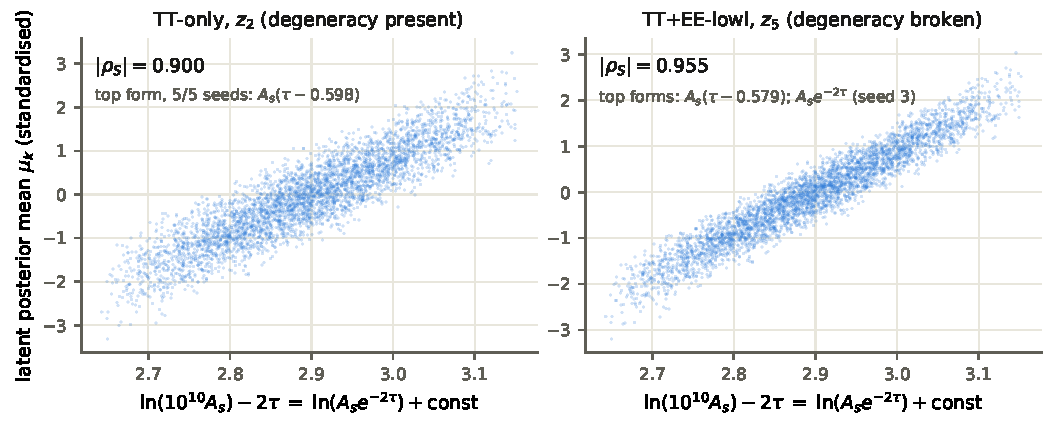
\includegraphics[width=\textwidth]{amplitude_scatter.pdf}
\caption{The amplitude latent of each checkpoint against the textbook
combination (computed \emph{only} for this figure; the search never sees it).
Points: 4\,000 of the 25k confirmatory-tier rows; $\rho_S$ is the Spearman
correlation on the full tier. The search, fed only raw $(\As,\tau)$, returns
the combination's first-order Taylor form $\As(\tau-c)$ with $c$ within
1.5--5\% of the predicted $\bar\tau+\tfrac12\approx0.570$, and (EE, seed 3)
the literal $\combo$.}
\label{fig:money}
\end{figure*}

The TT spectrum constrains $\As$ and $\tau$ above the reionization scale only
through $\combo$ \citep{planck2018}. Both checkpoints devote a latent to this
direction, and the blind search recovers it. Feeding the search raw
$(\As,\tau)$ only, the TT amplitude latent returns $\As(\tau-0.598)$ in 5/5
seeds (held-out MI $0.822$ nat, cross-seed spread $\pm0.025$); the EE amplitude
latent returns the $\As(\tau-0.579)$ family and, in one seed, the literal
$249.9\,\combo+0.118$ ($1.196\pm0.001$ nat). These \emph{are} the textbook
combination: the first-order Taylor expansion of $\combo$ about the prior mean
$\bar\tau$ predicts the affine form with $c=\bar\tau+\tfrac12\approx0.570$,
matching the discovered constants to 1.5--5\% (Fig.~\ref{fig:money}). That TT
returns only the affine form is structural, not seed luck: over the prior
$\tau\in[0.01,0.13]$, $e^{-2\tau}$ is 99.9\% linear (maximum deviation 0.52\%),
the two forms tie in MI, and parsimony deterministically prefers complexity 5
over 9. A regex scan over all Pareto-front equations finds the textbook
direction in 28/78 (TT) and 37/78 (EE) equations; the literal exponential
appears only in EE, whose latent is cleaner.

The $-2$ exponent itself is then read out four independent ways
(Table~\ref{tab:minus2}) --- including with all six parameters exposed and no
latent pre-selected, and including one readout that lives entirely in the
observable domain. A fifth, unsolicited appearance: the EE $\Hz$-latent's
\emph{residual} coordinate (stage 2, \S\ref{sec:hierarchy}) is literally
$\combo/\omB^2$ with ratio $-2.0000$, found blindly twice --- once by the
additive stage-2 run and again by the independent interaction-aware rerun.

Both regimes matter. In TT the degeneracy is \emph{present}: the single
amplitude latent is forced into the combination. In TT+low-$\ell$EE the
reionization bump breaks the degeneracy, the model \emph{could} separate
$\As$ from $\tau$ --- and its amplitude latent still organises as $\combo$.
The agreement of the forced and the emergent arm is the result.

\begin{table*}[t]
\centering\small
\caption{Four independent blind readouts of the reionization exponent
(textbook value $-2$), plus its unsolicited fifth appearance. Each row is a
different instrument on different data; none computes the textbook combination.}
\label{tab:minus2}
\begin{tabular}{@{}p{4.1cm}p{5.6cm}p{6.5cm}@{}}
\toprule
Readout & Instrument & Value \\
\midrule
1. Discovered forms & 2-input blind SR, $(\As,\tau)\to$ amplitude latent &
TT: $\As(\tau-0.598)$, 5/5 seeds; EE: $\As(\tau-0.579)$ + literal $\combo$;
affine $c$ matches Taylor prediction to 1.5--5\% \\
2. Derivative ratio & 6-input blind SR, all latents; $r=(\partial_\tau
f)/(\partial_{\lnAs} f)$ on top forms & $-1.974\pm0.018$ (TT);
$-1.993\pm0.008$ (EE) \\
3. Constant-ratio detector & frozen answer-agnostic ratio field
$\rho_{ij}=(\partial f/\partial u_i)/(\partial f/\partial u_j)$, cv $<5\%$ &
$(\tau,\lnAs)$ pair emerges with $r_\mathrm{raw}=-2.000$ (TT $z_4$, EE $z_5$
cards) \\
4. Decoder domain & decoder effect $d_k(\ell)$ decomposed onto data-driven
parameter templates & EE reionization bump: $r_\mathrm{dec}=a_\tau/a_{\lnAs}
=-1.87$ (TT collinear by mechanism; \S\ref{sec:structure}) \\
\addlinespace
5. (bonus) Residual reappearance & stage-2 SR on the EE $\Hz$-latent residual &
$f_2=\combo/\omB^{2}$, ratio $-2.0000$; found independently twice \\
\bottomrule
\end{tabular}
\end{table*}

\subsection{A validated card for every latent}
\label{sec:cards}

\begin{table*}[t]
\centering\small
\caption{Latent cards, both checkpoints (confirmatory-tier values). $f_1$: the
canonical primary coordinate, discovered blindly on the blindly selected
support $S^*$; $\etaS$: saturation of the support's own MI ceiling
($\etaS>1$ is possible within estimator tolerance); $\etapost$: fraction of the
information the stochastic latent stores, for $f_1$ alone and with the
discovered second coordinate $f_2$; $\RSR$: fraction of seeds recovering the
canonical form. Status is assigned by the frozen predicates.}
\label{tab:cards}
\begin{tabular}{@{}llllcccl@{}}
\toprule
$z$ & role (audit) & $f_1$ (canonical, blind) & $\etaS$ &
$\etapost(f_1)$ & $\etapost(f_1{+}f_2)$ & $\RSR$ & status \\
\midrule
\multicolumn{8}{@{}l}{\emph{TT-only (\texttt{lcdm\_tt\_beta3e-4}, $L=5$)}}\\
\addlinespace[2pt]
0 & $\omB$ & $\ns/\omB$ & 1.003 & 0.531 & 0.903 & 1.00 & primarily interpreted \\
1 & $\omC$ & $\Hz^2\ns^2\omB/(\As\omC^2)$ & 1.000 & 0.770 & 0.957 & 0.80 & primarily interpreted \\
2 & amplitude $(\As,\tau)$ & $\As/\log(\Hz(\omC+\tau))$ & 1.000 & 0.347 & 0.601 & 1.00 & primarily interpreted \\
3 & $\ns$ & $\ns+\omC$ & 0.997 & 0.447 & 0.838 & 1.00 & primarily interpreted \\
4 & $\Hz$ & $\As \Hz^2\omC\, e^{-2\tau}$ & 1.000 & 0.371 & 0.758 & 0.80 & primarily interpreted \\
\addlinespace[3pt]
\multicolumn{8}{@{}l}{\emph{TT+EE-lowl (\texttt{lcdm\_tt\_ee\_lowl}, $L=6$)}}\\
\addlinespace[2pt]
0 & $\omC$ / early ISW & $\omC/(\Hz\ns\omB)$ & 1.000 & 0.756 & 0.842 & 1.00 & \textbf{unresolved} \\
1 & $\Hz$ & $\Hz^2\omC$ & 1.000 & 0.348 & 0.663 & 1.00 & primarily interpreted \\
2 & $\omB$ & $\omB/\ns^2$ & 0.995 & 0.574 & 0.963 & 1.00 & primarily interpreted \\
3 & $\ns$ & $\log(\omB)/(\ns+\omC)$ & 0.992 & 0.493 & 0.864 & 0.80 & primarily interpreted \\
4 & $\tau$ (amplitude sector) & $-\As/(\tau-0.445)$ & 1.068 & 0.842 & 0.842 & 1.00 & primarily interpreted \\
5 & amplitude $(\As,\tau)$ & $\combo$ & 1.000 & 0.289 & 0.590 & 1.00 & primarily interpreted \\
\bottomrule
\end{tabular}
\end{table*}

\begin{figure*}[t]
\centering
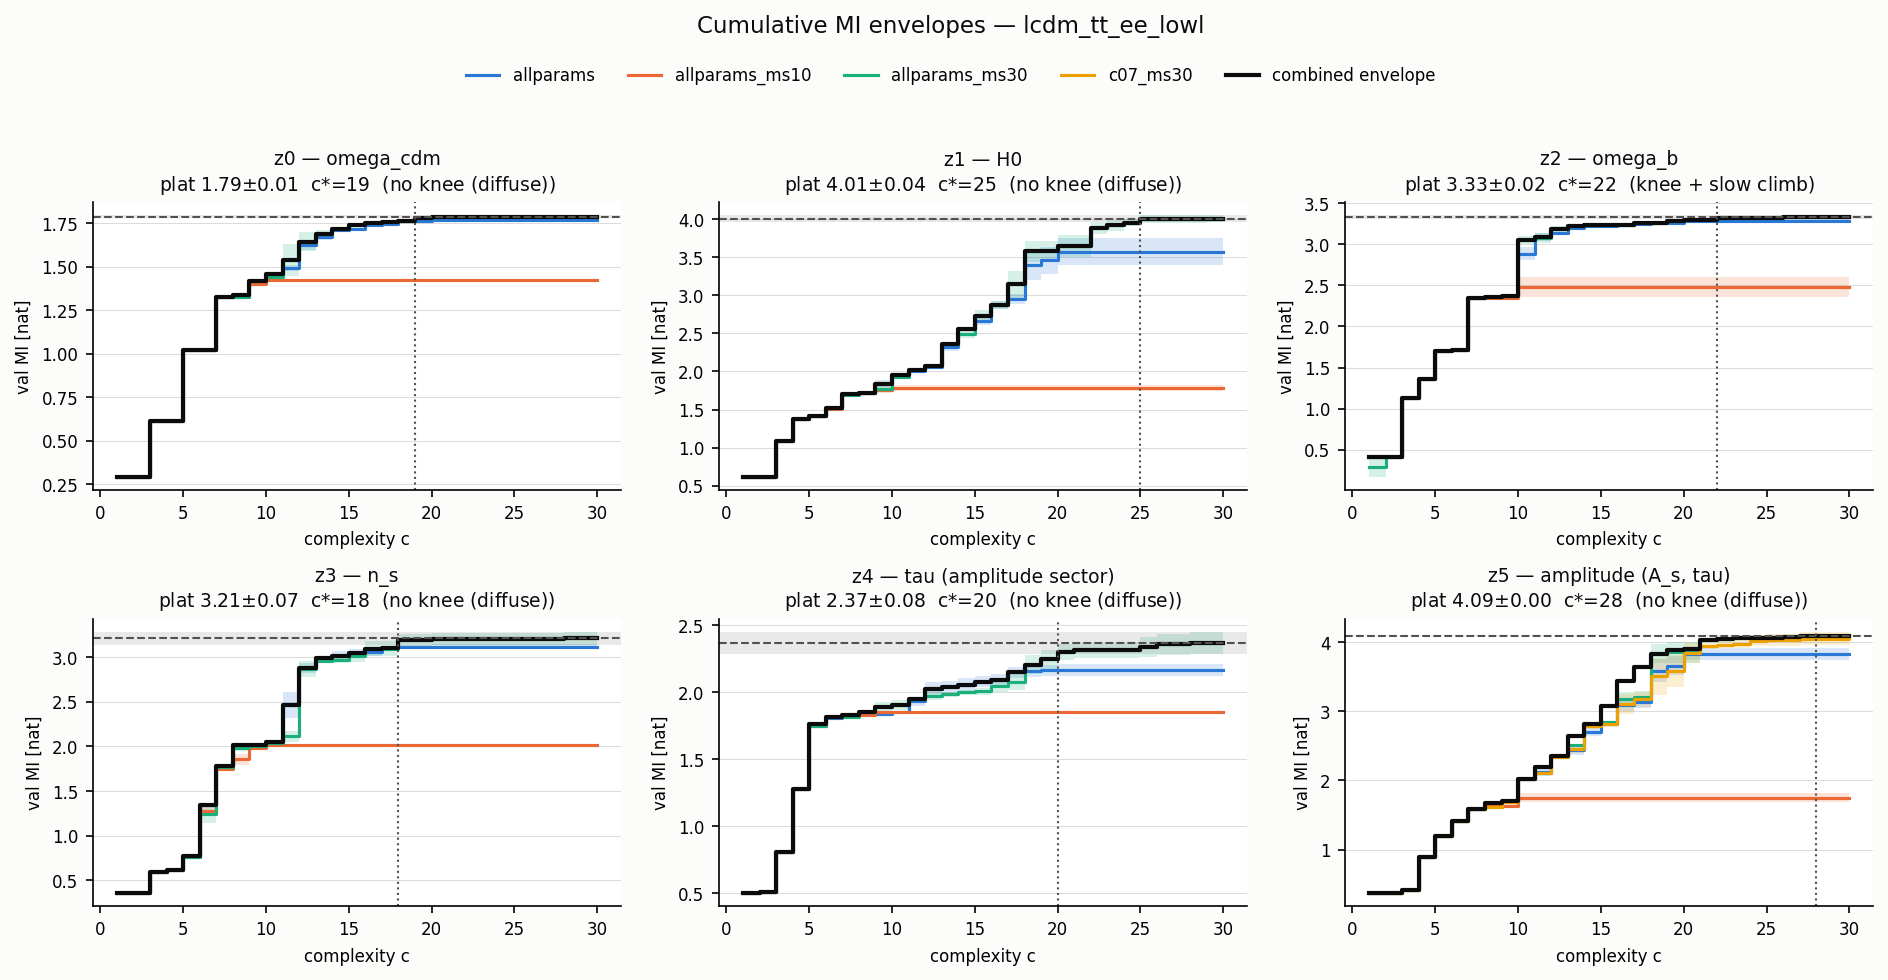
\includegraphics[width=0.92\textwidth]{knee_readout_lcdm_tt_ee_lowl_envelopes.png}
\caption{Cumulative Pareto envelopes (validation MI vs.\ expression
complexity), TT+EE-lowl checkpoint; the TT-only analogue is in the repository.
Plateaus span 1.79--4.18 nat, one-SE knees sit at complexity 18--28, and 10 of
11 latents' fronts are diffuse (no sharp knee) --- the information is spread
over complexity, one face of the non-terminating hierarchy of
\S\ref{sec:hierarchy}. Results are read at the knee, not at the front's argmax
(\S\ref{sec:objective}).}
\label{fig:envelopes}
\end{figure*}

Extending the frozen protocol from the amplitude control to all 11 latents
yields Table~\ref{tab:cards}. Three claims survive every gate:

\emph{Every latent has a one-dimensional symbolic primary coordinate that
saturates its own support} ($\etaS=0.99$--$1.07$ against ceilings from a blind
$2^6{-}1=63$-subset campaign) and recurs across search seeds ($\RSR\ge0.8$
everywhere, 8/11 at 1.00). The amplitude latents return $S^*=$ all six
parameters as a reproducible superset finding --- the all-parameter ceiling
genuinely beats $\{\As,\tau\}$ because shape-sector modulation of the latent is
real information. A post-closure, pre-registered rerun of the \emph{complete}
63-support grid at full protocol under a budget-matched readout later resolved
the three supports flagged as non-recurrent at the screen tier and bounded
input-set search dilution; its crossed outcome is reported with the negative
results (\S\ref{sec:negative}).

\emph{Every stage-1 residual is structured} ($R^2_\mathrm{res}=0.96$--$0.994$
against permutation nulls $\approx0$): no latent is a clean one-function
channel. Stage-2 search on the residuals (\S\ref{sec:hierarchy}) gives each
latent a discovered second coordinate, lifting $\etapost$ to 0.59--0.96.

\emph{One latent fails honestly.} EE $z_0$ has the weakest stage-2 account
($R^2\approx0.4$) and its joint level sets miss the frozen invariance bar
($\Einv=0.060$--$0.062$ vs.\ 0.05). The blocker is localised --- its residual
holds more than one coordinate's worth of structure --- and the card says so
rather than stretching a predicate.

\subsection{Structure of the codes}
\label{sec:structure}

\begin{figure}[tb]
\centering
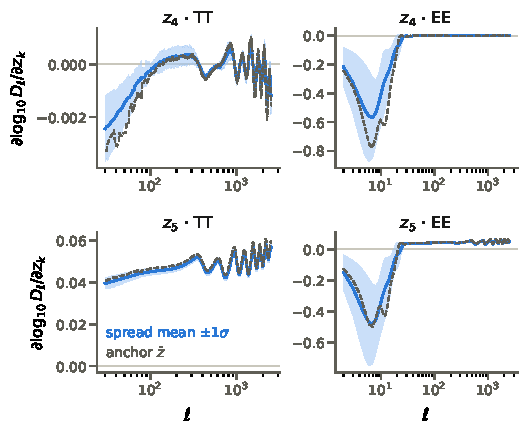
\includegraphics[width=0.98\columnwidth]{decoder_amplitude.pdf}
\caption{Decoder effect $d_k(\ell)=\partial\log_{10}D_\ell/\partial z_k$ for
the amplitude-sector latents of the TT+EE-lowl checkpoint (all 11 latents'
curves are in the repository). Solid: mean $\pm1\sigma$ over 64 posterior-mean
anchors; dashed: the central anchor. The low-$\ell$ EE reionization bump loads
almost exclusively on $z_4,z_5$ (right column; amplitude template mass
0.79--0.90), which is what makes the observable-domain readout
$r_\mathrm{dec}=-1.87$ of Table~\ref{tab:minus2} possible; template
decompositions achieve $R^2_W=0.988$--$1.000$ with
$\cos(a^*,g_j)=0.77$--$1.00$ against the symbolic-side signatures.}
\label{fig:decoder}
\end{figure}

Three model-level facts, all blind:

\emph{Degeneracy breaking has a latent-count fingerprint.} The raw-MI audit
alone shows one amplitude-sector latent in TT and two in TT+EE --- visible
before any regression. This is the physics: low-$\ell$ EE
($\propto\As\tau^2$) supplies the independent handle on $\tau$.

\emph{The EE amplitude sector is split, not duplicated.} Sparse-probe and
conditional-MI analysis shows $z_4$'s $\tau$-direction is carried by $z_4$
essentially alone, no redundant latent pair exists in either model (every
top-two carrier conditional is synergistic), and conditioning on $z_5$ raises
$z_1$'s information about $\combo$ from 0.013 to 0.473 nat.

\emph{Coordinates are latent-anchored, tails distributed.} Every $f_1$ is
linearly decodable from its own latent at rank-normal $R^2=0.88$--$0.95$, but
no card is axis-aligned; the second coordinates $f_2$ are genuinely distributed
across the code (own-latent $R^2=0.01$--$0.58$).

The decoder closes the loop in the observable domain
(Fig.~\ref{fig:decoder}): per-latent decoder responses $d_k(\ell)$ decompose
onto data-driven parameter templates, agree with the symbolic-side sensitivity
signatures, and, through the EE reionization bump, deliver the fourth $-2$
readout. In TT the same construction fails \emph{by mechanism} --- $\tau$ and
$\lnAs$ are collinear in $\ell\ge30$ TT template space --- which we document
rather than patch.

\subsection{The hierarchy does not terminate --- and the audits agree
quantitatively}
\label{sec:hierarchy}

Stage-2 blind SR on the cached residuals $e_1=\mu-h(f_1)$ (all six inputs,
five seeds) finds a recurrent $f_2$ for all 11 latents ($\RSR\ge0.80$; MI
against $e_1$ of 0.40--1.77 nat where shuffled-residual nulls give
$\le0.074$). Combined accounts $h(f_1)+g(f_2)$ reach $R^2(\mu)=0.955$--$0.998$
--- and the frozen stage-2 residual audit \emph{still} fails for all 11: the
encoder hierarchy does not terminate at two symbolic levels. This is a
statement about the representation, not the instruments, and it is robust: a
post-closure rerun exposing the stage-1 prediction $\hat f_1=h(f_1)$ as a
seventh input (so multiplicative amplitude$\times$shape interactions are
expressible) returns the identical canonical $f_2$ for 8/11 latents, upgrades
EE $z_0$'s $f_2$ to a unanimous interaction form without rescuing its card,
and shows the one registered additive-ansatz limit (TT amplitude latent,
deviation D-DoD-z2) is real structure --- the search keeps the $\tau$-bearing
form even when the interaction channel is available.

The interventional audit agrees with the calibration audit \emph{numerically},
not just in direction. Holding $f_1$ fixed and moving everything else, the
latent moves: $\Einv$ fails the frozen 0.05 rule for all 11 latents --- but
the failure magnitude is the structured residual itself,
$\Einv/(1-R^2_\mathrm{cal})\in[1.1,\,2.6]$ across all latents. Jointly holding
$(f_1,f_2)$ restores invariance for 7 of the 8 auditable latents (EE amplitude:
$0.226\to0.029$, passing the pre-registered gate on confirmatory data); the
three TT latents whose union support is all six parameters have no nuisance
direction left to test, and EE $z_0$ is the one joint failure
(\S\ref{sec:cards}).

\begin{table}[t]
\centering\small
\caption{Controls (condensed; full table in the repository). Real-signal
values in parentheses.}
\label{tab:controls}
\begin{tabular}{@{}p{4.55cm}p{3.15cm}@{}}
\toprule
Control & Result \\
\midrule
Shuffled-target SR, 2-input amplitude & 0.01--0.03 nat (real 0.82/1.20); no
textbook structure \\
Shuffled-target SR, all-params & $\le0.06$ nat on any control front \\
Stage-1 permutation nulls ($R^2$) & $p_{97.5}\approx-0.002$/$0.001$, all 11
latents \\
Shuffled-residual SR, stage 2 & 0.009--0.074 nat (real 0.40--1.77) \\
$\;$ + interaction-aware rerun & 0.010--0.053 nat \\
Level sets: shuffled-form $\Einv$ & 0.81--2.20 (pass bar 0.05) \\
Level sets: wrong-latent $\Einv$ & 0.2--2.8 (specificity) \\
Subspace shuffled probes & $R^2\approx0.000$; MI floors $\approx0.001$ nat \\
Positive control (gate G1) & known answer recovered \emph{and} its structured
residual reported \\
\bottomrule
\end{tabular}
\end{table}

\subsection{Negative results worth keeping}
\label{sec:negative}

The hyperparameter sweep (12 configurations $\times$ 3 seeds $\times$ 2
models) yields three reusable search-hygiene facts: (i) top-of-front MI
measures search capacity, not discovery --- maximum expression size alone
swings it 1.6$\to$4.05 nat while the winning composites differ structurally
seed to seed; (ii) the budget-matched MI at complexity $\le$10 is flat across
every knob ($\approx$1.89 nat TT / 2.02 EE) --- the leading-order discovery is
saturated at protocol settings, and the recovered physics is
hyperparameter-robust ($r\approx-1.97$ to $-2.00$ in every configuration);
(iii) a small search is not a shortcut to parsimony: the maxsize-10 search's
own front is \emph{worse} at complexity $\le$10 than the sliced maxsize-20
front (1.60 vs.\ 1.89 nat TT; 1.69 vs.\ 2.02 EE).

A fourth fact comes from a post-closure, pre-registered experiment (R-P4):
\emph{all} 63 supports rerun at full protocol (3\,465 grid cells, five seeds)
and read with a budget-matched statistic $M_S^{(c\le10)}$ under a frozen
select-then-confirm rule, alongside a sham-input control --- the
all-parameter search rerun with a seventh input that is a permuted copy of a
real parameter column, hence provably carrying zero information. The two legs
cross. On TT the sham input demonstrably dilutes the search
($\Delta_\mathrm{sham}=-0.040\pm0.013$ nat pooled over 75 paired runs), yet
only one strict subset beats all-six on the held-out tier ($z_3$,
$+0.090\pm0.062$); on EE the sham costs nothing ($+0.014\pm0.013$), yet five
of six latents confirm a strict-subset advantage --- three substantive,
$+0.09$ to $+0.13$ nat, the strongest at $z_4$ where $\{\omC,\tau,\As,\ns\}$
beats all-six by $+0.126\pm0.047$; the other two pass the frozen $+1$-SE rule
at magnitudes $\le0.003$ nat and are read as negligible. The sham symbol appears in $0.0\%$ of
best-at-budget forms in either model. The practical reading: budget-matched
damage from searching on the full input set is real but small
($\lesssim0.13$ nat), and where subsets win the gain comes from removing
specific weakly-coupled true inputs (a distractor effect), not from a smaller
search space per se. The three screen-tier support-recurrence flags are
thereby resolved (TT $z_0$: all-six stands; EE $z_3$, $z_4$: genuine subset
advantages); no card status or headline number changes.

\section{Limitations and scope}
\label{sec:limits}

\textbf{All claims are per-checkpoint.} Five search seeds establish
\emph{search} stability; stability under VAE retraining ($R_\mathrm{model}$)
was not run --- it requires GPU retraining in the parent repository and
remains executable later without touching any frozen threshold. The amplitude
family's recurrence across two different architectures and data regimes, with
the latent-count fingerprint matching the physics, is partial cross-model
evidence, not a substitute. Further: the symbolic hierarchy is non-terminating
at the two levels probed (plus the enriched interaction ansatz); a third level
was not attempted. EE $z_0$ remains unresolved with a localised blocker. The
TT decoder readout of the $-2$ is structurally unavailable (template
collinearity), so $r_\mathrm{dec}$ is EE-only. Estimator caveats are handled
by design: decisions ride on $\eta$ ratios, not raw MI, with bootstrap errors
and data-processing-inequality checks throughout.

\section{Conclusion}
\label{sec:conclusion}

A symbolic-regression pipeline whose only reward is bijection-invariant mutual
information, wrapped in a pre-registered freeze--validate--unblind protocol,
recovers the CMB amplitude--reionization combination $\ln(\combo)$ from two
$\beta$-VAE encoders with the $-2$ exponent read out four independent ways,
and returns a falsifiable symbolic card for every latent --- including one
honest failure and an encoder hierarchy that does not terminate at two
symbolic levels. Nothing in the ladder of Table~\ref{tab:ladder} is specific
to the CMB: it is a recipe any scientific-VAE interpretation study can run,
every instrument shipping its own null.

\paragraph*{Reproducibility.} All searches ($\approx$4\,600 PySR runs,
$\approx$7\,600 CPU core-hours), consolidated deliverables, frozen thresholds,
deviation register, and the per-latent cards are in the repository
(\texttt{cmb-lcdm-sr}); every number above is regenerable from
\texttt{experiments/*.json} and is a confirmatory-tier (T2) value.

\begingroup
\footnotesize
\begin{thebibliography}{9}
\setlength{\itemsep}{1pt}

\bibitem{piras2025}
D.~Piras, L.~Herold, L.~Lucie-Smith, and E.~Komatsu,
``$\Lambda$CDM and early dark energy in latent space: a data-driven
parametrization of the CMB temperature power spectrum,''
arXiv:2502.09810 (2025).

\bibitem{cranmer2023}
M.~Cranmer,
``Interpretable machine learning for science with PySR and
SymbolicRegression.jl,''
arXiv:2305.01582 (2023).

\bibitem{piras2023}
D.~Piras et al.,
``A robust estimator of mutual information for deep learning
interpretability,''
Mach.\ Learn.: Sci.\ Technol.\ \textbf{4}, 025006 (2023).

\bibitem{klein2005}
J.~R.~Klein and A.~Roodman,
``Blind analysis in nuclear and particle physics,''
Annu.\ Rev.\ Nucl.\ Part.\ Sci.\ \textbf{55}, 141 (2005).

\bibitem{schmidt2009}
M.~Schmidt and H.~Lipson,
``Distilling free-form natural laws from experimental data,''
Science \textbf{324}, 81 (2009).

\bibitem{cranmer2020}
M.~Cranmer et al.,
``Discovering symbolic models from deep learning with inductive biases,''
NeurIPS 33 (2020), arXiv:2006.11287.

\bibitem{class2011}
D.~Blas, J.~Lesgourgues, and T.~Tram,
``The Cosmic Linear Anisotropy Solving System (CLASS) II: approximation
schemes,''
JCAP \textbf{07}, 034 (2011).

\bibitem{planck2018}
Planck Collaboration,
``Planck 2018 results. VI. Cosmological parameters,''
Astron.\ Astrophys.\ \textbf{641}, A6 (2020).

\bibitem{higgins2017}
I.~Higgins et al.,
``$\beta$-VAE: learning basic visual concepts with a constrained variational
framework,''
ICLR (2017).

\end{thebibliography}
\endgroup

\end{document}
